\documentclass[12px]{article}

\title{Ultima lezione di teoria del nostro caro papi}
\date{2024-05-30}
\author{Federico De Sisti}

\usepackage{amsmath}
\usepackage{amsthm}
\usepackage{mdframed}
\usepackage{amssymb}
\usepackage{nicematrix}
\usepackage{amsfonts}
\usepackage{tcolorbox}
\tcbuselibrary{theorems}
\usepackage{xcolor}
\usepackage{cancel}

\newtheoremstyle{break}
  {1px}{1px}%
  {\itshape}{}%
  {\bfseries}{}%
  {\newline}{}%
\theoremstyle{break}
\newtheorem{theo}{Teorema}
\theoremstyle{break}
\newtheorem{lemma}{Lemma}
\theoremstyle{break}
\newtheorem{defin}{Definizione}
\theoremstyle{break}
\newtheorem{propo}{Proposizione}
\theoremstyle{break}
\newtheorem*{dimo}{Dimostrazione}
\theoremstyle{break}
\newtheorem*{es}{Esempio}

\newenvironment{dimo}
  {\begin{dimostrazione}}
  {\hfill\square\end{dimostrazione}}

\newenvironment{teo}
{\begin{mdframed}[linecolor=red, backgroundcolor=red!10]\begin{theo}}
  {\end{theo}\end{mdframed}}

\newenvironment{nome}
{\begin{mdframed}[linecolor=green, backgroundcolor=green!10]\begin{nomen}}
  {\end{nomen}\end{mdframed}}

\newenvironment{prop}
{\begin{mdframed}[linecolor=red, backgroundcolor=red!10]\begin{propo}}
  {\end{propo}\end{mdframed}}

\newenvironment{defi}
{\begin{mdframed}[linecolor=orange, backgroundcolor=orange!10]\begin{defin}}
  {\end{defin}\end{mdframed}}

\newenvironment{lemm}
{\begin{mdframed}[linecolor=red, backgroundcolor=red!10]\begin{lemma}}
  {\end{lemma}\end{mdframed}}

\newcommand{\icol}[1]{% inline column vector
  \left(\begin{smallmatrix}#1\end{smallmatrix}\right)%
}

\newcommand{\irow}[1]{% inline row vector
  \begin{smallmatrix}(#1)\end{smallmatrix}%
}

\newcommand{\matrice}[1]{% inline column vector
  \begin{pmatrix}#1\end{pmatrix}%
}

\newcommand{\C}{\mathbb{C}}
\newcommand{\K}{\mathbb{K}}
\newcommand{\R}{\mathbb{R}}


\begin{document}
	\maketitle
	\newpage
	\section{Boh}
	\textbf{Osservazioni}\\
	1. Metrico $=$ euclideo\\
	2. Per distinguere l'ellisse non degenere a punti reali da quella a punti immaginari, si può usare il seguente criterio
	\[
		A=(a_{ij})^2_{i,j=0} \ \ A_0=(a_{ij})^2_{i,j=1}
	.\] 
	$tr A_0 \det A $ \begin{cases}
		>0 \text{ellisse a punti immaginari}\\
		<0 \text{ellisse a punti reali}
	\end{cases}\\
$ \displaystyle\lambda_1 x^2 + \lambda_2 y^2 + \frac{\det A}{\det A_0} = 0$\\
Non ci sono soluzioni reali se e solo se $\lambda_1 ($ o  $\lambda_2)$ hanno lo stesso segno di $\det A$, è equivalente dire
\[
tr A_0 \det A >0
.\] 
\section{geometria delle coniche euclidee}
\textbf{Ellissi}\\
$\displaystyle \frac{x^2}{a^2} + \frac {y^2}{b^2}=1 \ \ \ \ \ a\geq b>0$\\
 $a = b \ \ \ x^2 + y^2 = a^2$ circonferenza di centro l'origine e rango $a$ \\
 Il  supporto dell'ellisse è chiuso e limitato, infatti esso è centrato nel rettangolo delimitato dalle rette $x\pm a, \ \ y=\pm b$
  \[
	  supp \ \ \ell \subset \{ (x,y)\in\R^2 : |x|\leq a , \ |y| \leq b\}
 .\] 
\begin{center}
	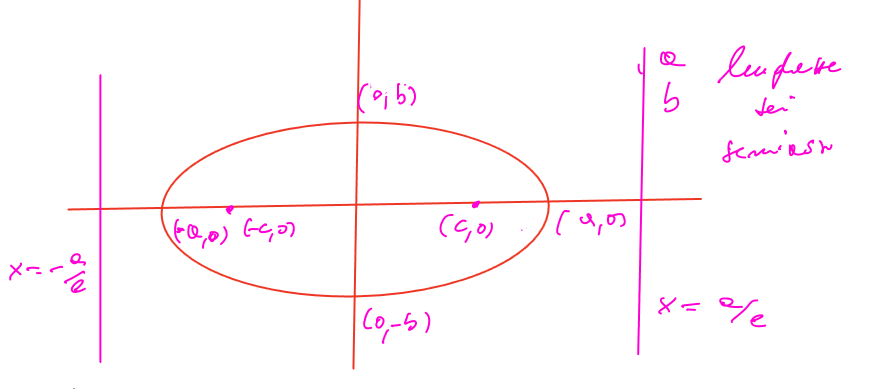
\includegraphics[scale=.45]{ellisse.png}
\end{center}
  $\displaystyle\frac {x^2}{a^2} + \frac{y^2}{b^2} \leadsto y=\frac b a \sqrt{a^2-x^2}, \ \ y = =\frac b a \sqrt{a^2-x^2}$ \\
  \begin{defi}
	  $c = \sqrt{a^2-b^2} \ \ (\pm c, 0) $ fuori di $\ell$
	   \[
		   e = \frac c a \ \ \ \text{eccentriche di }\ell
	  .\] 
  \end{defi}
  \textbf{Nota}\\
  $0 \leq e < 1, \ \ e = 0 \Leftrightarrow\lee$ circonferenza
  \[
	  x =\pm \frac a c  \text{manca qualcosa}
  .\] 
  \textbf{Iperbole}\\
  $\displaystyle\frac {x^2}{e^2} - \frac{y^2}{b^2} = 1 \ \ a > 0, b > 0$\\
\begin{center}
	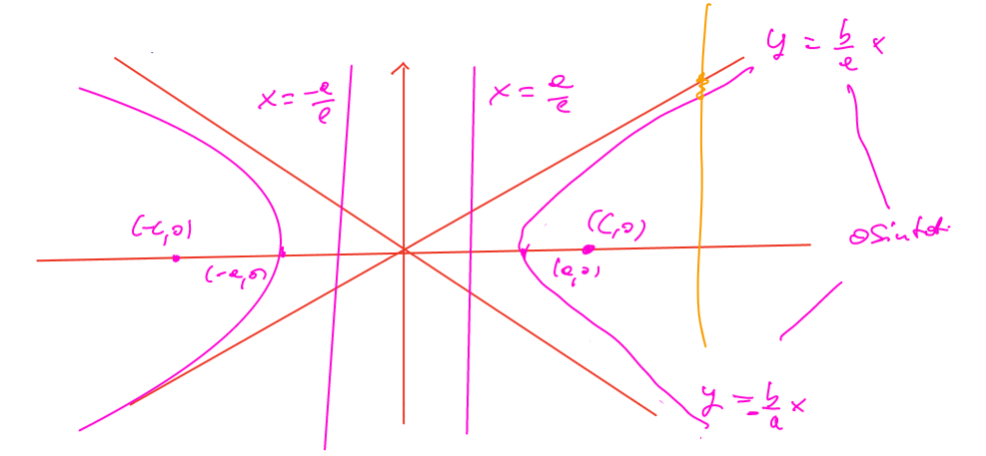
\includegraphics[scale=.45]{iperbole.png}
\end{center}
  \begin{defi}
	  $c = \sqrt{a^2 + b^2} \ \ (\pm c,0)$ fuochi di $\ell$ 
	   \[
		   e = \frac c a \ \ \ \ \text{eccentricità } e>1
	  .\] 
	  \[
		  x = \pm \frac a c \ \ \text{ direttrici}
	  .\] 
  \end{defi}
  \textbf{Parabola}\\
  $y^2 = 2 px \ \ p>0\ \ \ y = \pm\sqrt{2px}$\\
\begin{center}
	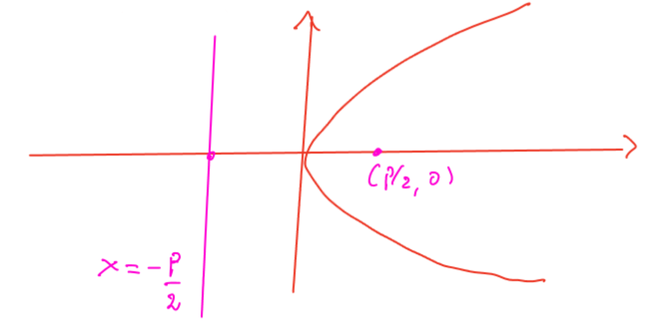
\includegraphics[scale=.45]{parabola.png}
\end{center}
\begin{defi}
	Il fuoco di $\ell$ \ \ \ $(\frac p 2 , 0)$
	 \[
		 \text{ direttrice } \ \ x = -\frac  p 2 \ \ \ e = 1 \ \ \text{eccentricità}
	.\] 
\end{defi}
\begin{prop}
	L'ellisse (1) e l'iperbole (2) hanno per supporto il luogo dei punti le cui distanze dai due fuochi ha somma (rispettivamente differenza) costante (rispettivamente costante in valore assoluto) uguale a $2a$
\end{prop}
\begin{prop}
	L'ellisse (1), l'iperbole (2), la parabola (3) hanno per supporto il luogo dei punti le cui distanze da un fuoco e dalla relativa direttrice hanno rapporto costante uguale ad $e$ l'eccentricità della conica
\end{prop}
\begin{dimo}[proposizione 1]
	Siano $F, F'$ i fuochi, di coordinate $(c,0),(-c,0)$ rispettivamente.
	Imponiamo la condizione
	\[
	|d(P,F)\pm d(P,F')| = 2a
	.\] 
	Se $P$ ha  coordinate $(x,y)$ risulta \[
		|\sqrt{(x-c)^2+y^2}\pm\sqrt{(x+c)^2 + y^2}| = 2a \ \ \cirlcedast\circledast
	.\] 
	Elevando due volte al quadrato, otteniamo 
	\[
		\frac{x^2}{a^2} + \frac{y^2}{a^2-c^2} = 1 \ \ \cirlcedast
	.\] 
	Se $c = \sqrt{a^2 - b^2} \leadsto \frac{x^2}{a^2} + \frac{y^2}{b^2} =1$ ellisse\\
	Se $c = \sqrt{a^2 + b^2} \leadsto \frac{x^2}{a^2} - \frac {y^2}{b^2} = 1$ iperbole\\
	Per concludere, osserviamo che il luogo rappresentato da $\circledast$ è precisamente (1) nel caso dell'ellisse e (2) nel caso dell'iperbole\\
	A questo scopo, basta osservare che il procedimento è reversibile a meno di affinità di segni nei radicali. Però la conclusione\\
	\[
		c < a \ \ \text{ è compatibile col prendere} + \text{nell'equazione} \circledast\circledast
	.\] 
	\[
		c > a \ \ \text{ è compatibile col prendere} - \text{nell'equazione} \circledast\circledast
	.\] 
\end{dimo}
\begin{dimo}[proposizione 2]
	La condizione che definisce il luogo cercato è 
	\[
		\frac{d(P,F)}{d(P,r)}=e
	.\] 
	$ P = (x,y)$
	\begin{tikzpicture}[remember picture, overlay]
		\node[xshift=120mm,yshift=-84mm,anchor=north west] at (current page.north west){%
		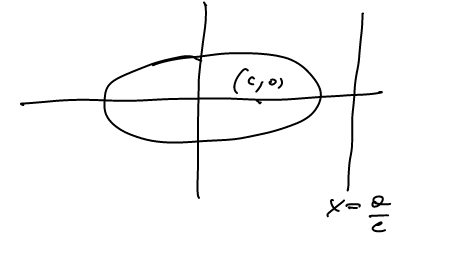
\includegraphics[width=40mm]{ellisse_prop.png}}
	\end{tikzpicture}
	 \[
		 \frac{\sqrt{(x-c)^2+y^2}}{|x-\frac{a}{c}|}=e
	.\] 
	$(x-c)^2 + y^2 = e^2 (x-\frac a e)^2$ \\
	$x^2 - 2cx + c^2 + y^2 = e^2x^2 - 2aex + a^2$\\
	$x^2 (1-e^2) + y^2 = \cancel{2(c - ea)x} + a^2 - c^2$ dato che $c = \frac e a$ e  $e = \frac c a$\\\
	$(1 - \frac {c^2}{a^2})x^2 + y^2 = b^2$ \\
	$\frac{a^2 - c^2}{a^2}x^2 + y^2 = b^2$\\
	$\frac{b^2}{e^2}x^2 + y^2 = b^2$\\
	$\frac{x^2}{a^2} + \frac{y^2}{b^2} = 1$\\
	Gli altri cambi per l'iperbole sono analoghi e lasciati per esercizio
\end{dimo}
\ \hline\ \\
$\pro^2$  \\
\begin{center}
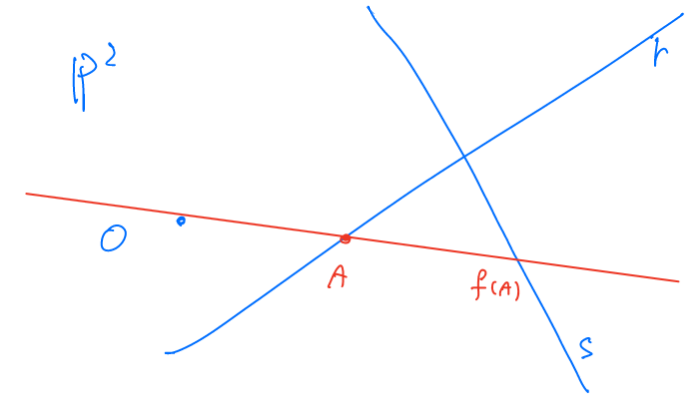
\includegraphics[scale=.5]{prospettivita_2.png}
\end{center}
Più in generale, dati $S_1,S_2$ spazi proiettivi tali che $\dim S_1 = \dim S_2 = k$ in $\pro^n$, e  $H$ sottospazio $H\cap S_1 = H\cap S_2 =\emptyset$ e $\dim H = n - k -1 $, la prospettività di centro $M$ è la restrizione a $S_1$ della proiezione su $S_2$ di centro $H$ ; è un isomorfismo $S_1 \rightarrow S_2$\\
\textbf{Esercizio}\\
Siano in $\pro^3$ $T_1$ il piano $x_3 = 0$ e $T_2$ il piano $x_0+2x_1-3x_2=0$\\
\[
	Q = [0,1,-1,1], \ \ f: T_1 \rightarrow T_2 \ \ \text{ di centro } Q
.\] 
Trova equazioni cartesiane dell'immagine di $r=T_1\cap T_3$ dove $T_3:x_0+x_1=0$\\
Risulta $f(r) = L(Q,r)\cap T_2$\\
$r$ ha equazioni  \begin{cases}
	x_3=0\\
	x_0+x_1=0
\end{cases}\\
Il fascio di piani di asse $r$ ha equazione
\[
	\lambda(x_0+x_1)+\mu x_3=0 \ \ \ \ \ [\lambda,\mu]\in\pro^1(\R)
.\]
Imponendo il passaggio per $[0,1,-1,1]$ otteniamo\\
\[
	\lambda + \mu =0 \ \ \ \ [\lambda,\mu] = [1,-1]
.\] 
$L(Q,r):x_0+x_1-x_3=0 \ \ f(r) \ \  \begin{cases}
	x_0+x_1-x_3=0\\
	x_0+2x_1-3x_2
\end{cases}$
\ \\ \hline\ \\ 
Siano $r,s\subseteq\pro^2(\R)$ rette distinte, $A=r\cap s$ e $f:r \rightarrow s$ un isomorfismo proiettivo allora.\\
(a) $f$ è una prospettività se e solo se $f(A) = A$\\
(b) Se  $f(A)\neq A , $ esiste una retta $t$ in $\pro^2$ e due prospettività $g: r \rightarrow t, \ \ h : t \rightarrow s$ tale che
\[
 f = h\circ g
.\] 
(c) Ogni proiettività $p:r \rightarrow r$ è composizione di al più tre prospettività
\\
$(a)$ per costruzione una prospettività fissa il punto $A$\\
\begin{center}
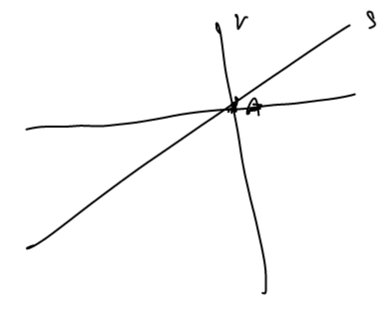
\includegraphics[scale=.5]{prospettivita_3.png}
\end{center}
 Viceversa, supponiamo che $f:r \rightarrow s$ sia tale che $f(A) = A$ 
\begin{center}
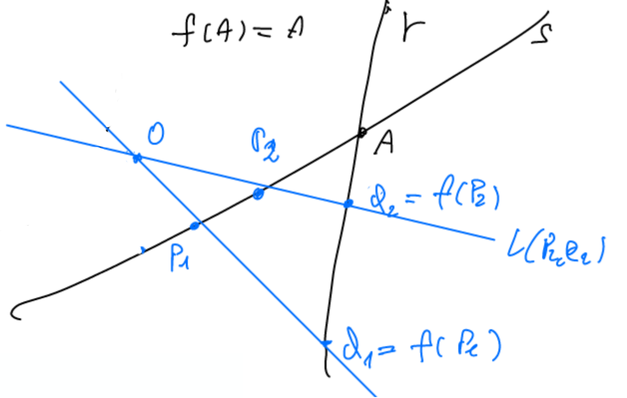
\includegraphics[scale=.5]{prospettivita_4.png}
\end{center}
 $L(P_1,Q_1)\cap L(P_2,Q_2) = 0 \not \in r\cup s$\\
 Se $g$ è la prospettività di centro $O$, risulta $g(A) = A,\ \  g(P_1)=Q_1, \ \ g(P_2)=Q_2$\\
 Ma $A,P_1,P_2, \ \ \ A,Q_1,Q_2$ sono punti in posizione generale\\
 e pertanto, per il teorema fondamentale, $f=g$

\end{document}

